\section{Sequenzielle Systeme}
\subsection{Zustandstabelle}
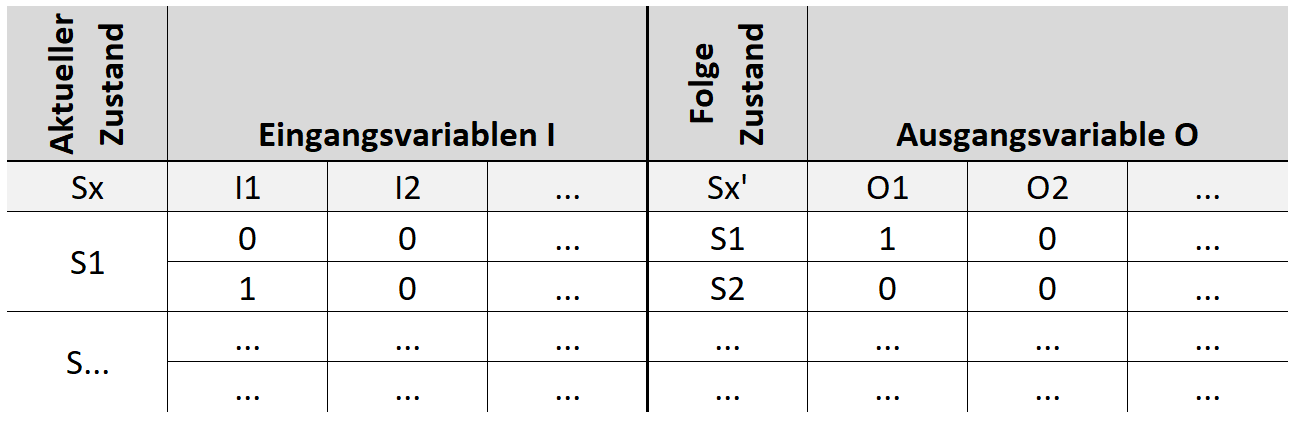
\includegraphics[width=\columnwidth,keepaspectratio=true]{./Images/zustandstabelle.png}

\subsection{Zustandsdiagramm}
\begin{minipage}{\textwidth}	
	\begin{minipage}{0.25\textwidth}
		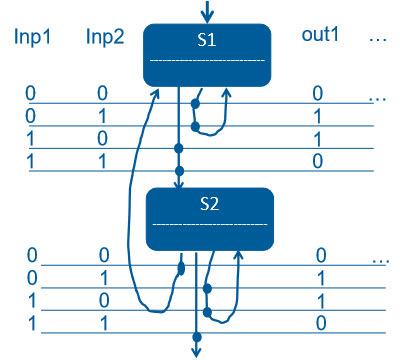
\includegraphics[width=\linewidth,keepaspectratio=true]{./Images/zustandsdiagram.png}
	\end{minipage}%%% to prevent a space
	\begin{minipage}{0.25\textwidth}
		\begin{enumerate}
			\item Zustände zeichnen 
			\item Initial Zustand bestimmen
			\item Eingänge systematisch auflisten
			\item Zustandsübergänge bestimmen
			\item Ausgänge einzeichnen
		\end{enumerate}
	\end{minipage}
\end{minipage}

\subsection{Zustandscodierung}
\noindent\textbf{Binär Codierung}\\
Kompakt und weniger FlipFlop als One-Hot/Cold.

\begin{tabular}{ll}
Anzahl Speicherstellen $k$:& $k = \left\lceil \frac{\log_{10}(p)}{\log_{10}(2)}\right\rceil$\\
Max Anzahl Zustände $p$:& $p <= 2^k$ \\
Möglichen Zustandscodierungen $q$:& $q = \frac{(2^k)!}{(2^k - p)!}$ 
\end{tabular}\\ 

\noindent\textbf{Gray Code}\\ 
Spezialfall von Binärcodierung, es wechselt jeweils nur 1 Bit zwischen den Zuständen. \\

\noindent\textbf{One-Hot/Cold Codierung}\\
One-Hot (nur eine 1 pro Zustand), One-Cold (nur eine 0 pro Zustand) sind schneller als Binär-Codierungen.

\begin{tabular}{ll}
	Anzahl Speicherstellen $k$:& $k = p$\\
	Max. Anzahl Zustände $p$:& $p = k$ \\
	Möglichen Zustandscodierungen $q$:& $q = p!$ 
\end{tabular}
